%!TEX root = /Users/ego/Boulot/TKZ/tkz-tab/doc/TKZdoc-tab-main.tex   
% $Id$  
% 20 / 02 /2009 v1.00c TKZdoc-tab-tangente    
%  Created by Alain Matthes on 2010-02-23.
%  Copyright (c) 2010 __Collège Sévigné__. All rights reserved.
% 

\section{Tangente horizontale : \addbs{tkzTabTan} et  \addbs{tkzTabTanFrom}}
\subsection{Définition de \tkzcname{tkzTabTan}}

\begin{NewMacroBox}{tkzTabTan}{\oarg{local options}\{Début\}\{Fin\}\{Position\}\{Image\}}

\begin{tabular}{lllc}
\toprule
\texttt{arguments}   & \texttt{défaut}    & \texttt{définition}         \\
\midrule
\IargName{tkzTabTan}{Début}&|no default|&rang de l'origine de la flèche   \\
\IargName{tkzTabTan}{Fin}&|no default|& rang de l'extrémité de la flèche   \\
\IargName{tkzTabTan}{Position}  & |no default|  & rang de l'antécédent     \\
\IargName{tkzTabTan}{Image}  & |no default|  & valeur de l'image     \\
\bottomrule
\end{tabular}

\medskip
\noindent\emph{Il s'agit de savoir sur quelle flèche, on va positionner la tangente. \tkzname{Début} et \tkzname{Fin} sont les rangs des valeurs qui déterminent les extrémités de la flèche. \tkzname{Position} est le rang de la valeur qui correspond à la tangente. \tkzname{Image} est la valeur que l'on peut joindre à la tangente (ordonnée du point de contact).}

\medskip
\begin{tabular}{lllc}
\toprule
\texttt{options}   & \texttt{défaut}    & \texttt{définition}                    \\
\midrule
\IoptName{tkzTabTan}{pos}     & |below| & position de la valeur                  \\
\bottomrule
\end{tabular}

\medskip
\noindent\emph{Il existe une option \tkzname{pos} qui permet de positionner cette valeur sous la tangente.\\}

\end{NewMacroBox}


\subsection{Utilisation des arguments}

\subsubsection{Palier}
La flèche débute pour la valeur initiale $0$ donc de rang $1$ et se termine pour $+\infty$, valeur de rang $3$.  La tangente est ici en $x=1$ soit la valeur de rang $2$.

\begin{tkzexample}[vbox]
\begin{tikzpicture}
 \tkzTab[espcl=6]{$x$/1,$f'(x)$ /1, $f$/3}%
 {$0$ , $1$ , $+\infty$}%
 {d , + , 0 , + , }
 {D- / $-\infty$ , R /  , +/ $+\infty$}%
 \tkzTabTan{1}{3}{2}{\scriptsize $2$}
\end{tikzpicture}
\end{tkzexample}  

\subsubsection{Tangente à l'extrémité d'un intervalle}
Dans l'exemple ci-dessous, la flèche débute pour la valeur initiale $0$ donc de rang $1$ et se termine pour $1$, valeur de rang $2$. La tangente est ici en $x=1$ soit la valeur de rang $2$. Il faut remarquer que la macro \tkzcname{tkzTabTan} s'applique à la ligne de variations qui la précède.

La valeur $0$ de l'image de $1$ par $f$ n'est pas indiquée dans \tkzcname{tkzTabVar}. Elle serait sous les flèches représentant la tangente, aussi elle est passée comme argument de \tkzcname{tkzTabTan} avec l'option \tkzname{pos=below}.

\begin{tkzexample}[vbox]
\begin{tikzpicture}
 \tkzTabInit[espcl=6]{$x$ /1,$f'(x)$/1,$f$/2}{$0$,$1$,$+\infty$}%
 \tkzTabLine{t , + , z , - , }%
 \tkzTabVar{-/ $-1$ , +/  , -/$-\infty$ }
 \tkzTabTan[pos=below]{1}{2}{2}{$0$}
\end{tikzpicture}
\end{tkzexample}  

\subsection{Utilisation des options}

\subsubsection{\texttt{\textcolor{red}{pos}} : position de la valeur} 

\begin{tkzexample}[vbox]
\begin{tikzpicture}
 \tkzTabInit[espcl=5]{$x$/1,$f''{x}$/1,$f'(x)$/2,$f(x)$/2}{$0$,$1$,$+\infty$}%
 \tkzTabLine{d,+,0,-,}%
 \tkzTabVar{-/ $-\infty$  ,+/ ,-/$-\infty$}
 \tkzTabTan[pos=below]{1}{2}{2}{$0$}
 \tkzTabVar{+/ $+\infty$ , R/ , -/ $0$}
 \tkzTabTan{1}{3}{2}{$1$}
\end{tikzpicture}
\end{tkzexample}  

\subsubsection{Variations imbriquées} 
\begin{tkzexample}[vbox]
\begin{tikzpicture}
  \tkzTabInit[espcl=3]
  {$x$      /1,
   $f''(x)$ /1,
    $f'$    /3,
     $f$    /3}%
  {$0$ , $\alpha$ , $1$ , $\beta$, $+\infty$ }%
  \tkzTabLine {d , +,  , + , z , - , , - }%
  \tkzTabVar {-/ $-1$  / , R/ ,+/ , R/ , -/ $-\infty$ }
  \tkzTabIma[draw]{1}{3}{2}{0}
  \tkzTabIma[draw]{3}{5}{4}{0}
  \tkzTabTan[pos]{1}{3}{3}{$2$}
  \tkzTabVar{+/ $+\infty$ , - / , R/,+/  , -/ $0$ }
  \tkzTabTan[]{1}{2}{2}{$1$}
  \tkzTabTan[pos=below]{2}{4}{4}{$2$}
\end{tikzpicture}
\end{tkzexample}  


\subsection{Définition de \textcolor{red}{tkzTabTanFrom}}

\begin{NewMacroBox}{tkzTabTanFrom}{\oarg{local options}\{Début\}\{Fin\}\{Position\}\{Image\}}

\begin{tabular}{lllc}
\toprule
\texttt{arguments}   & \texttt{défaut}    & \texttt{définition}         \\
\midrule
\IargName{tkzTabTanFrom}{Début} & |no default|  & rang de l'origine de la flèche       \\
\IargName{tkzTabTanFrom}{Fin} & |no default|  & rang de l'extrémité de la flèche     \\
\IargName{tkzTabTanFrom}{Position} & |no default|  & nom d'un point        \\
\IargName{tkzTabTanFrom}{Image} & |no default|  & valeur de l'image        \\
\bottomrule
\end{tabular}

\medskip
\noindent\emph{La position est donnée  par le nom d'un point ou d'un node.}

\medskip
\begin{tabular}{lllc}
\toprule
\texttt{options}   & \texttt{défaut}    & \texttt{définition}       \\
\midrule
\IoptName{tkzTabTan}{pos}     & |below| & position de la valeur      \\
\bottomrule
\end{tabular}


\end{NewMacroBox}
\subsection{Le nom est défini par le tableau}
Le nom du node qui correspond à $\alpha$ est ici \tkzname{N21} (antécédent de rang 2, premier filet sous la valeur.)
\begin{tkzexample}[vbox,small]
\begin{tikzpicture}
\tkzTabInit[ espcl=6]
{ $x$              /1,
  $f'(x)$          /1,
  $f$              /3}
{ $0$ ,  $\alpha$ , $+\infty$ }%
\tkzTabLine { , ,+, , }%
\tkzTabVar{-/ $-1$ , R , +/ $+1$ /}%
\tkzTabTanFrom[pos=below]{1}{3}{N21}{$0$}
\end{tikzpicture}
\end{tkzexample}  

\subsection{Le nom est donné par l'utilisateur avec l'option \texttt{\textcolor{red}{remember}}}

\begin{tkzexample}[vbox,small]
\begin{tikzpicture}
\tkzTabInit[ espcl=4]
{ $x$              /1,
  $f''(x)$         /1,
  $f'$          /2,
  Signe de $f'(x)$ /2,
  $f$           /3}
{ $0$ , $1$ , $\alpha$ , $+\infty$ }%
\tkzTabLine {d,+,0,-, ,- }%
\tkzTabVar
{-/ $1$       ,
 +/           ,
 R/           ,
 -/ $-\infty$ }%
\tkzTabTan[pos,remember=v1]{1}{2}{2}{$2$}%
\tkzTabVal[remember=v2]{2}{4}{0.5}{}{0}%
\tkzTabLine { ,, +,, z,- }%
\tkzTabVar
{-/ $-\infty$ ,
 R/           ,
 +/           ,
 -/ $0$       }
\tkzTabImaFrom[]{1}{3}{v1}{0}%
\tkzTabImaFrom[]{3}{4}{v2}{}%
\tkzTabTanFrom[pos=below]{3}{4}{v2}{$1$}
\end{tikzpicture}
\end{tkzexample}  


\endinput